
%(BEGIN_QUESTION)
% Copyright 2003, Tony R. Kuphaldt, released under the Creative Commons Attribution License (v 1.0)
% This means you may do almost anything with this work of mine, so long as you give me proper credit

Some common components of three-phase motor control circuits are shown here in the following illustrations.  These include {\it fuses}, a {\it contactor}, and an {\it overload} assembly:

$$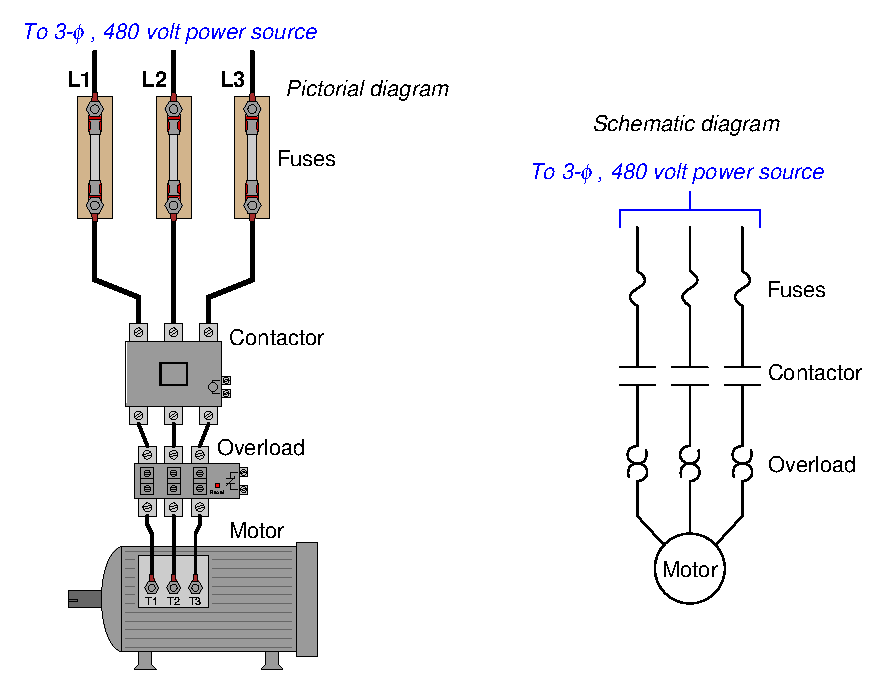
\includegraphics[width=15.5cm]{i01444x01.eps}$$

Fuses protect the power wiring from gross overcurrent conditions such as what might happen if there were an accidental phase-to-phase short-circuit inside the motor.  The contactor is nothing more than a big relay with three normally-open contacts to send power to the motor, serving to start and stop the motor on command with a 120 volt signal to its coil.  

\vskip 10pt

The overload block, however, is a little more mysterious.  Its three ``heater'' elements (looking like back-to-back ``question mark'' symbols in the schematic diagram) carry the motor's current from the contactor to the motor terminals.  These resistive heaters are designed to become warm under normal operating conditions, just as the motor itself will become slightly warm under normal conditions from resistive power losses in its windings.

If the motor ever becomes too warm as a result of overloading (slight overcurrent), the overload heaters (which will also be too warm due to the overcurrent) will trigger a small thermally-operated switch contact to spring open.  Connection terminals for this small switch contact may be seen on the right-hand side of the overload block in the pictorial diagram.

\vskip 10pt

Explain how the overload heaters may be used to automatically shut the motor off and prevent damage.

\underbar{file i01444}
%(END_QUESTION)





%(BEGIN_ANSWER)

If you thought the overload heaters would open up like fuses in the event of an overload condition (becoming too warm) to directly interrupt motor current, you have made a very common error!  Don't feel bad, though -- I won't tell anyone.

In order for the overload assembly to automatically shut down the motor, its small switch must be connected to something.  I'll let you figure out what that something is!

%(END_ANSWER)





%(BEGIN_NOTES)

The OL contact may be wired in series with the contactor coil to tell the contactor to open in the event of an overload.

$$\includegraphics[width=15.5cm]{i01444x02.eps}$$

When the overload ``heaters'' become excessively warm from overcurrent, they trigger the opening of the ``OL'' contact, thus stopping the motor.  The heaters do not take the place of regular overcurrent protection devices (circuit breakers, fuses), but serve a different purpose entirely.  It is the task of the overload heaters to protect the {\it motor} against overcurrent by mimicking the thermal characteristics of the motor itself.  Circuit breakers and fuses, on the other hand, protect the wiring conveying power to the motor!
 
An interesting way to explain the function of overload heaters is to refer to them as {\it analog models} of the motor windings.  They are designed such that at any given current level, they will take as long to heat up and reach their trip point as the real motor itself will take to heat up to a point of impending damage.  Likewise, they also cool off at the same rate as the real motor cools off when no power is applied.  Overload heaters are like small motor-models with a thermostat mechanism attached, to trip the overload contact at the appropriate time.  It is an elegant concept, and quite practical in real motor control applications.

%INDEX% Final Control Elements, motor: overload heater

%(END_NOTES)


